\documentclass[13pt,a4paper]{report}
\usepackage[margin=0.6in]{geometry}
\usepackage{fancybox}
\usepackage[utf8]{inputenc}
\usepackage[vietnamese,main=english]{babel}
\usepackage{multicol}
\usepackage{tabularx}
\usepackage{lmodern}
\usepackage{indentfirst}
\usepackage{float}
\usepackage{enumitem}
\usepackage{afterpage}
\usepackage[super]{nth}
\usepackage{titlesec}
\usepackage{bigdelim}
\usepackage[titles]{tocloft}
\usepackage{makecell}
\usepackage{arydshln}
\usepackage{perpage} %the perpage package
\usepackage{graphicx}
\usepackage{caption}
\usepackage{minted}
\usepackage{amsmath}
\usepackage{gensymb}
\usepackage{tikz}
\usepackage{circuitikz}
\usepackage{pgfplots}
\usepackage{cancel}
\usepackage{xurl}
\usepackage[bottom]{footmisc}
\usepackage[font=footnotesize,labelfont={scriptsize}]{subfig}
\usepackage{wrapfig}
\usepackage{latexsym,amssymb,amsmath}
%\usepackage{algpseudocode}
\usepackage{tocvsec2}
\usepackage{fancyref}
\usepackage{bookmark}
\usepackage{hyperref}
\usepackage[nameinlink,noabbrev]{cleveref}

\newcolumntype{Y}{>{\centering\arraybackslash}X}

\PassOptionsToPackage{hyphens}{url}

\newcommand{\instbit}[1]{\mbox{\scriptsize #1}}
\newcommand{\instbitrange}[2]{~\instbit{#1} \hfill \instbit{#2}~}

% New column types to use in tabular environment for instruction formats.
% Allocate 0.18in per bit.
\newcolumntype{I}{>{\centering\arraybackslash}p{0.18in}}
% Two-bit centered column.
\newcolumntype{W}{>{\centering\arraybackslash}p{0.36in}}
% Three-bit centered column.
\newcolumntype{F}{>{\centering\arraybackslash}p{0.54in}}
% Four-bit centered column.
\newcolumntype{Y}{>{\centering\arraybackslash}p{0.72in}}
% Five-bit centered column.
\newcolumntype{R}{>{\centering\arraybackslash}p{0.9in}}
% Six-bit centered column.
\newcolumntype{S}{>{\centering\arraybackslash}p{1.08in}}
% Seven-bit centered column.
\newcolumntype{O}{>{\centering\arraybackslash}p{1.26in}}
% Eight-bit centered column.
\newcolumntype{E}{>{\centering\arraybackslash}p{1.44in}}
% Ten-bit centered column.
\newcolumntype{T}{>{\centering\arraybackslash}p{1.8in}}
% Twelve-bit centered column.
\newcolumntype{M}{>{\centering\arraybackslash}p{2.2in}}
% Sixteen-bit centered column.
\newcolumntype{K}{>{\centering\arraybackslash}p{2.88in}}
% Fifteen-bit centered column.
\newcolumntype{U}{>{\centering\arraybackslash}p{2.7in}}
% Twenty-bit centered column.
\newcolumntype{L}{>{\centering\arraybackslash}p{3.6in}}
% Twenty-five-bit centered column.
\newcolumntype{J}{>{\centering\arraybackslash}p{4.5in}}


\makeatletter
\pgfcircdeclarebipole{}{\ctikzvalof{bipoles/vsourceam/height}}{vsourceAM}{\ctikzvalof{bipoles/vsourceam/height}}{\ctikzvalof{bipoles/vsourceam/width}}{%
  \pgfsetlinewidth{\pgfkeysvalueof{/tikz/circuitikz/bipoles/thickness}\pgfstartlinewidth}
   \pgfpathellipse{\pgfpointorigin}{\pgfpoint{0}{\pgf@circ@res@up}}{\pgfpoint{\pgf@circ@res@left}{0}}
   \pgfusepath{draw}
   \pgfscope
       \pgftransformxshift{0.6*\ctikzvalof{bipoles/vsourceam/margin}\pgf@circ@res@left}
       \pgftext[rotate=-\pgf@circ@direction]{$+$}
       \pgfusepath{draw}
   \endpgfscope
   \pgfscope
       \pgftransformxshift{0.6*\ctikzvalof{bipoles/vsourceam/margin}\pgf@circ@res@right}
       \pgftext[rotate=-\pgf@circ@direction]{$-$}
       \pgfusepath{draw}
   \endpgfscope
}
\makeatother

\MakePerPage{footnote} %the perpage package command
\usetikzlibrary{shapes,positioning,arrows,calc,automata}

\newcommand*\justify{%
  \fontdimen2\font=0.4em% interword space
  \fontdimen3\font=0.2em% interword stretch
  \fontdimen4\font=0.1em% interword shrink
  \fontdimen7\font=0.1em% extra space
  \hyphenchar\font=`\-% allowing hyphenation
}
\renewcommand\cftchapafterpnum{\vskip-2pt}
\renewcommand\cftsecafterpnum{\vskip-2pt}

\renewcommand{\theequation}{\arabic{equation}}

% FLOW CHART
\tikzstyle{startstop} = [rectangle, rounded corners, minimum width=3cm, minimum height=1cm,text centered, draw=black, fill=red!30]
\tikzstyle{io} = [trapezium, trapezium left angle=70, trapezium right angle=110, minimum width=3cm, minimum height=1cm, text centered, draw=black, fill=blue!30]
\tikzstyle{process} = [rectangle, minimum width=3cm, minimum height=1cm, text centered, draw=black, fill=orange!30, text width=4cm]
\tikzstyle{decision} = [diamond, aspect=2.5, minimum width=3cm, minimum height=1cm, text centered, draw=black, fill=green!30]
\tikzstyle{arrow} = [thick,->,>=stealth]

% CHAPTER FORMAT
\titleformat{\chapter}%[display]
{\bfseries\fontsize{25}{30}\selectfont\raggedright}% Format and size of title text
{\llap{%
    \rule[-8pt]{6cm}{1.18cm}\rule{6pt}{0pt}}% Black box to the left, lowered 6pt. The end rule is a horisontal space.
  \llap{% Number also to the left, on top of the black box.
    \fontsize{22}{44}\selectfont\color{white}\thechapter\rule{10pt}{0pt}}}{0pt}{}{}

\counterwithin{figure}{section}
\renewcommand{\thefigure}{\arabic{chapter}.\arabic{section}.\alph{figure}}

\renewcommand{\thetable}{\arabic{table}}

\renewcommand\labelitemi{$-$}
  
\titleformat{\section}
  {\LARGE\bfseries}{}{}{}
\renewcommand\thesection{\arabic{section}.}
\renewcommand\thesubsection{\arabic{subsection}}
\makeatletter
\renewcommand*\l@section{\@dottedtocline{1}{1.5cm}{2em}}
\renewcommand\section{\@startsection {section}{1}{-1em}%
  {-3.5ex \@plus -1ex \@minus -.2ex}%
  {2.3ex \@plus.2ex}%
  {\normalfont\Large\bfseries}}
\def\sectionmark#1{%
      \markright {\MakeUppercase{#1}}}
\makeatother

\titleformat{\subsection}
  {\normalfont\bfseries}{\thesubsection.}{0.5em}{}
\renewcommand\cftsubsecaftersnum{.} 
\renewcommand\thesubsection{\alph{subsection}}

\addto{\captionsenglish}{%
  \renewcommand{\bibname}{References}
}

%\addtocontents{toc}{\setcounter{tocdepth}{2}}
%\addtocontents{lof}{\vskip -1.6cm}
%\addtocontents{lot}{\vskip -1.6cm}

    
% TOC settings
\renewcommand\cftchapnumwidth{2.8em}
\renewcommand\cftsecnumwidth{3em}
\renewcommand\cftsecindent{3em}
\renewcommand\cftsubsecindent{5em}
\renewcommand\thechapter{\Roman{chapter}}
    
%\titleformat{\chapter}[display]{\normalfont\huge\bfseries}{}{0pt}{\Huge}
\newcommand{\hsp}{\hspace{20pt}}
%\titleformat{\chapter}[hang]{\Huge\bfseries}{\thechapter\hsp\textcolor{gray75}{|}\hsp}{0pt}{\Huge\bfseries}
\titleformat*{\subsubsection}{\large\bfseries}
%\titlespacing*{\chapter}{0pt}{0pt}{0pt}
    
\newcolumntype{P}[1]{>{\centering\arraybackslash}p{#1}}
\newcolumntype{C}{>{\centering\arraybackslash}p{4em}}
    
\setlist[itemize]{noitemsep, topsep=0pt}
%\AtBeginEnvironment{multicols}{\RaggedRight}

\titlespacing*{\chapter}{0pt}{0pt}{20pt}

\newcommand\Chapter[2]{\chapter
  [#1\text{: }\hfil\hbox{}\protect\linebreak{\itshape#2}]%
  {#1\\[-0.75ex]\Large#2}%
  \markboth{\MakeUppercase{\chaptername\ \thechapter.\ #1}}{}%
}


\def\doubleoverline#1{\overline{\overline{#1}}}

\captionsetup[subfloat]{labelformat=empty}

\begin{document}
%Trang bìa 1
\fontsize{13pt}{18pt}\selectfont
\begin{titlepage}
\thispagestyle{empty}
\thisfancypage{%đóng khung trang này
\setlength{\fboxsep}{0pt}% 8pt là độ dày của đường viền
\fbox}{} % phần nội dung sau là tương tự như đã làm
\

\begin{center}
\begin{large}
HO CHI MINH CITY UNIVERSITY OF TECHNOLOGY $-$ VNU HCMC
\end{large} \\
\begin{large}
OFFICE FOR INTERNATIONAL STUDY PROGRAM
\end{large} \\
\begin{large}
FACULTY OF ELECTRICAL AND ELECTRONIC ENGINEERING
\end{large} \\
\textbf{--------------------  *  --------------------}\\[4cm]

\includegraphics[scale=0.1]{logobk.png}\\[1cm]
{\fontsize{20pt}{1}\selectfont DIGITAL SYSTEMS (LAB)}\\
{\fontsize{20pt}{1}\selectfont AN ENHANCED PROCESSOR}\\[2.5cm]
\end{center}

\begin{otherlanguage}{vietnamese}
\begin{tabbing}
	\hspace{3.5cm}Lecturer  \ \ \ \ \=: \textbf{\parbox[t]{9cm}{Mr. Nguyễn Tuấn Hùng}}\\
	\hspace{3.5cm}Subject \>: \textbf{\parbox[t]{12cm}{Digital Systems}}\\
	\hspace{3.5cm}Class \>: \textbf{\parbox[t]{9cm}{TT06}}\\
	\hspace{3.5cm}Name \>: \textbf{\parbox[t]{9cm}{
		Lương Triển Thắng}}\\
	\hspace{3.5cm}Student ID \>: \textbf{\parbox[t]{9cm}{
		2051194}}\\[40pt]
\end{tabbing}
\end{otherlanguage}

\vspace{2.25cm}
\begin{center}
{\fontsize{13pt}{1}\selectfont Ho Chi Minh City, \nth{21} June, 2022}
\end{center}
\end{titlepage}

\tableofcontents

\setminted{fontsize=\normalsize}

\chapter{Introduction}
In computing and computer science, a processor or processing unit is an electrical component (digital circuit) that performs operations on an external data source, usually memory or some other data stream. Based on the von Neumann architecture, they contain at least a control unit (CU), an arithmetic logic unit (ALU), and processor registers.

The world's first processor had introduced by Intel in the late 1971, named Intel 4004. It is a 4-bit processor with 12-bit address width. In 1975, a new game changer appreared, MOS Technology 6502, with 8-bit data width, 16-bit address width. It was `the heart' of most consumer personal computers, game consoles in the late 70s and 80s, including the Apple I, Apple II, Atari 7800, Commodore 64, Commodore VIC-20, Nintendo Entertainment System (NES), etc.

After years of development, numerous of instruction set architectures (ISAs) have been created. In 2022, there are some popular ISAs which are in used and development, such as:
\begin{itemize}
\item x86-64: 2001, org. 1978, Intel/AMD
\item MIPS: 1981
\item PowerISA: 1990, PowerPC
\item ARM: 1983, ARM/Raspberry/Qualcomm/...
\item RISC-V: 2010
\item ARM64: 2011, Apple/Nvidia/Qualcomm/Samsung/...
\end{itemize}

In this project, I will introduce two processors with two different ISAs.
\begin{itemize}
\item A nine-bit processor: followed Lab5, Lab6 instructions
\begin{itemize}[label={$+$}]
\item 8 instructions $\Rightarrow$ too few.
\item 9-bit data width $\Rightarrow$ one bit more than a word (8 bits), awkward.
\item 7-bit address width $\Rightarrow$ maximum of 128 addresses (16 bytes).
\item [$\Rightarrow$] Inefficient.
\end{itemize}

\item An eight-bit processor
\begin{itemize}[label={$+$}]
\item 21 instructions, 8 reserved.
\item 8-bit data width.
\item 16-bit address width $\Rightarrow$ up to 65536 addresses (8KB).
\end{itemize}
\end{itemize}

The source code for this project is rather large, I would not attached into this report. The link for the source code is present in the last chapter.


\Chapter{An enhanced processor}{A 9-bit processor}
According to instructions of Lab5 and Lab6, the details of the `enhanced processor' would be described in below.

\section{Registers}
\begin{center}
\begin{tabular}{|c|c|c|}
\hline 
Register & Width (bits) & Purpose \\ 
\hline 
R0 - R6 & 9 & General \\ 
\hline 
R7 & 9 & PC \\ 
\hline 
\end{tabular} 
\end{center}

\section{Instruction types}
Normal and Misc type of instruction requires only one instruction input.

Immediate type requires immediate value which successive with the instruction input.
\subsection{Normal}
\vspace{-0.4in}
\begin{center}
\begin{tabular}{R@{}R@{}R@{}R@{}}
\\
&
\instbitrange{8}{6} &
\instbitrange{5}{3} &
\instbitrange{2}{0} \\
\cline{2-4}
mv &
\multicolumn{1}{|c|}{000} &
\multicolumn{1}{c|}{DR} &
\multicolumn{1}{c|}{SR} \\
\cline{2-4}

add &
\multicolumn{1}{|c|}{010} &
\multicolumn{1}{c|}{RX} &
\multicolumn{1}{c|}{RY} \\
\cline{2-4}

sub &
\multicolumn{1}{|c|}{011} &
\multicolumn{1}{c|}{RX} &
\multicolumn{1}{c|}{RY} \\
\cline{2-4}

ld &
\multicolumn{1}{|c|}{100} &
\multicolumn{1}{c|}{DR} &
\multicolumn{1}{c|}{BaseR} \\
\cline{2-4}

st &
\multicolumn{1}{|c|}{101} &
\multicolumn{1}{c|}{SR} &
\multicolumn{1}{c|}{BaseR} \\
\cline{2-4}

mvnz &
\multicolumn{1}{|c|}{110} &
\multicolumn{1}{c|}{DR} &
\multicolumn{1}{c|}{SR} \\
\cline{2-4}

\end{tabular}
\end{center}

\subsection{Immediate}
\vspace{-0.4in}
\begin{center}
\begin{tabular}{R@{}R@{}R@{}R@{}I@{}U@{}}
\\
&
\instbitrange{8}{6} &
\instbitrange{5}{3} &
\instbitrange{2}{0} &
&
\instbitrange{8}{0} \\
\cline{2-4}
\cline{6-6}
mvi &
\multicolumn{1}{|c|}{001} &
\multicolumn{1}{c|}{DR} &
\multicolumn{1}{c|}{any}&
&
\multicolumn{1}{|c|}{imm9} \\
\cline{2-4}
\cline{6-6}
\end{tabular}
\end{center}

\subsection{Misc}
\vspace{-0.4in}
\begin{center}
\begin{tabular}{R@{}R@{}R@{}R@{}}
\\
&
\instbitrange{8}{6} &
\instbitrange{5}{3} &
\instbitrange{2}{0} \\
\cline{2-4}
halt &
\multicolumn{1}{|c|}{111} &
\multicolumn{1}{c|}{any} &
\multicolumn{1}{c|}{any} \\
\cline{2-4}
\end{tabular}
\end{center}

\section{Instruction details}
\begin{center}
\begin{tabular}{|c|c|c|c|c|}
\hline 
Instruction & Opcode & Operation & Cycles & Assembler format \\ 
\hline 
mv & 000 & \texttt{DR <= SR} & 1 & mv DR, SR \\ \hline 
mvi & 001 & \texttt{DR <= imm9} & 2 & mv DR, imm9 \\ \hline 
add & 010 & \texttt{RX <= RX + RY} & 3 & add RX, RY \\ \hline 
sub & 011 & \texttt{RX <= RX - RY} & 3 & sub RX, RY \\ \hline 
ld & 100 & \texttt{DR <= mem[BaseR]} & 2 & ld DR, BaseR \\ \hline 
st & 101 & \texttt{mem[BaseR] <= SR} & 3 & st SR, BaseR \\ \hline 
mvnz & 110 & \texttt{DR <= SR if G /= 0} & 2 or 3 & mvnz DR, SR \\ \hline 
halt & 111 & Halt the processor & $\infty$ & halt \\ \hline 
\end{tabular} 
\end{center}

\section{Transition table}
\begin{center}
\begin{tabular}{|c|c|c|c|}
\hline 
 & $T_1$ & $T_2$ & $T_3$ \\ 
\hline 
mv & \makecell{$RY_{out}$ = `1' \\ $RX_{in}$ = `1' \\ \textbf{done} = `1'} &  &  \\ \hline
mvi & \makecell{incr = `1' \\ $addr_{in}$ = `1' \\ $R7_{in}$ = `1'} & \makecell{$DIN_{out}$ = `1' \\ $RX_{in}$ = `1' \\ \textbf{done} = `1'} &  \\ \hline
add & \makecell{$RX_{out}$ = `1' \\ $A_{in}$ = `1'} & \makecell{$RY_{out}$ = `1' \\ $G_{in}$ = `1'} & \makecell{$G_{out}$ = `1' \\ $RX_{in}$ = `1' \\ \textbf{done} = `1'} \\ \hline
sub & \makecell{$RX_{out}$ = `1' \\ $A_{in}$ = `1'} & \makecell{$RY_{out}$ = `1' \\ $G_{in}$ = `1' \\ AddSub = `1'} & \makecell{$G_{out}$ = `1' \\ $RX_{in}$ = `1' \\ \textbf{done} = `1'} \\ \hline
ld & \makecell{$RY_{out}$ = `1' \\ $addr_{in}$ = `1'} & \makecell{$DIN_{out}$ = `1' \\ $RX_{in}$ = `1' \\ \textbf{done} = `1'} &  \\ \hline
st & \makecell{$RY_{out}$ = `1' \\ $addr_{in}$ = `1'} & \makecell{$RX_{out}$ = `1'  \\ $Dout_{in}$ = `1'} & \makecell{W = `1' \\ \textbf{done} = `1'} \\ \hline
mvnz & $G_{out}$ = `1' & done = zero & \makecell{$RY_{out}$ = `1' \\ $RX_{in}$ = `1' \\ \textbf{done} = `1'}  \\ \hline
halt & \makecell{\textbf{halt} = `1'} &  &  \\ \hline
\end{tabular} 
\end{center}

\section{Note}
A register contains 7 bits, while an address uses 7 bits to define, so source address of ld and destination address of st only uses BaseR[6:0].

In ld, Base[8:7] will define the load source, `00' for memory, `10' for KEY, `11' for SW.

In st, Base[8:7] will define the store destination, `00' for memory, `10' for LED.

\section{Assembler}
For ease of writing machine code for memory, I wrote a small program in Python assemble machine code.

Below is the example of a multiplier program which takes two inputs (address \#50 and SW), after calculating the product, it will store into address \#52 then output to LED.

I will use this to demo the processor in the next section.

\subsection*{Input assembly file}
\begin{minted}{nasm}
% R1 <= M[50]
mvi   R1, #50
ld    R1, R1

% R2 <= SW (600 in oct)
mvi   R4, #384
ld    R4, R4

% R0 <= R1 * R4
mvi   R2,#1
mv    R5,R7
add   R0, R1
sub   R4, R2
mvnz R7, R5

% M[52] <= R0
mvi R1, #52
st R0, R1

% R1 <= M[52]
mvi   R1, #52
ld    R1, R1

% LED (200 in oct) <= R1
mvi R6, #128
st R1, R6

halt

data 50, #12
\end{minted}

\subsection*{Output memory file}
\begin{minted}{vhdl}
WIDTH=9;
DEPTH=128;

ADDRESS_RADIX=UNS;
DATA_RADIX=OCT;

CONTENT BEGIN
	[0..127]	:	000;
	0	:	110;	-- mvi   R1, #50;
	1	:	062;
	2	:	411;	-- ld    R1, R1
	3	:	140;	-- mvi   R4, #384;
	4	:	600;
	5	:	444;	-- ld    R4, R4
	6	:	120;	-- mvi   R2,#1;
	7	:	001;
	8	:	057;	-- mv    R5,R7
	9	:	201;	-- add   R0, R1
	10	:	342;	-- sub   R4, R2
	11	:	675;	-- mvnz R7, R5
	12	:	110;	-- mvi R1, #52;
	13	:	064;
	14	:	501;	-- st R0, R1
	15	:	110;	-- mvi   R1, #52;
	16	:	064;
	17	:	411;	-- ld    R1, R1
	18	:	160;	-- mvi R6, #128;
	19	:	200;
	20	:	516;	-- st R1, R6
	21	:	700;	-- halt
	50	:	014;	-- data 50, #12
END;
\end{minted}

\section{Demonstration}
According to the program above and the value of SW = 000001000 = 8, the expected output R0 = R1 = $96_{10}$ = $060_{16}$ = LED = $001100000_2$

\begin{figure}[H]\centering
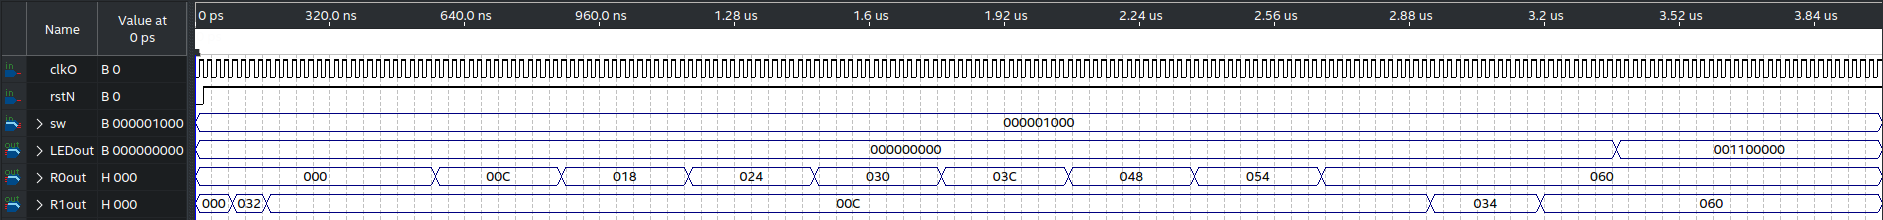
\includegraphics[scale=0.28]{images/9bit_waveform.png}
\end{figure}

\section{Conclusion}
The processor can run simple programs, but it would be a hassle when dealing with more complex programs that require large memory ($>$ 16 bytes), specialized instruction such as compare, branch, bitwise not, bitwise and,...

Thus, I came up with a better solution with describe in Chapter 3.

\Chapter{A better approach}{An 8-bit processor, but better}

\section{Registers}
The processor has 10 local registers. Registers R5 and R6 are the high and low index registers, H contains first 8 bits of a 16 bits value, L contains last 8 bits of a 16 bits value, these registers use in HL required instructions.

\begin{center}
\begin{tabular}{|c|c|l|}
\hline 
Register & Width (bits) & Purpose \\ 
\hline 
R0 & 8 & General \\ 
R1 & 8 & General \\ 
R2 & 8 & General \\ 
R3 & 8 & General \\ 
R4 & 8 & General \\ 
R5/H & 8 & General/High index register\\ 
R6/L & 8 & General/Low index register \\ 
R7 & 8 & General/in-out value \\ 
flags & 4 & less-equal-greater-carry \\ 
PC & 16 & Program counter \\ 
\hline 
\end{tabular} 
\end{center}

\section{Input/output devices}
\begin{center}
\begin{tabular}{|c|c|c|}
\hline 
devid (dd) & Input & Output \\ 
\hline 
00 & KEY & LED \\ 
\hline 
01 & SW & 8-bit decimal output to 7-segment display \\ 
\hline 
10 & n/a & 16-bit decimal output to 7-segment display \\ 
\hline 
11 & n/a & 16-bit hexadecimal output to 7-segment display\\ 
\hline 
\end{tabular} 
\end{center}

\section{Instruction types}
\subsection{RY-imm8}
\subsubsection{RY (mode 0)}
\vspace{-0.4in}
\begin{center}
\begin{tabular}{F@{}E@{}W@{}S@{}I@{}T@{}S@{}}
\\
&
\instbitrange{7}{4} &
\instbit{3} &
\instbitrange{2}{0} &
&
\instbitrange{7}{3} &
\instbitrange{2}{0} \\
\cline{2-4}
\cline{6-7}
mv & \multicolumn{1}{|c|}{0000} & \multicolumn{1}{c|}{0} & \multicolumn{1}{c|}{DR}& & \multicolumn{1}{|c}{00000} & \multicolumn{1}{|c|}{SR} \\ \cline{2-4} \cline{6-7}
add & \multicolumn{1}{|c|}{0001} & \multicolumn{1}{c|}{0} & \multicolumn{1}{c|}{RX}& & \multicolumn{1}{|c}{00000} & \multicolumn{1}{|c|}{RY} \\ \cline{2-4} \cline{6-7}
sub & \multicolumn{1}{|c|}{0010} & \multicolumn{1}{c|}{0} & \multicolumn{1}{c|}{RX}& & \multicolumn{1}{|c}{00000} & \multicolumn{1}{|c|}{RY} \\ \cline{2-4} \cline{6-7}
mul & \multicolumn{1}{|c|}{0011} & \multicolumn{1}{c|}{0} & \multicolumn{1}{c|}{SR1}& & \multicolumn{1}{|c}{00000} & \multicolumn{1}{|c|}{SR2} \\ \cline{2-4} \cline{6-7}
cmp & \multicolumn{1}{|c|}{0110} & \multicolumn{1}{c|}{0} & \multicolumn{1}{c|}{SR1}& & \multicolumn{1}{|c}{00000} & \multicolumn{1}{|c|}{SR2} \\ \cline{2-4} \cline{6-7}
and & \multicolumn{1}{|c|}{1001} & \multicolumn{1}{c|}{0} & \multicolumn{1}{c|}{RX}& & \multicolumn{1}{|c}{00000} & \multicolumn{1}{|c|}{RY} \\ \cline{2-4} \cline{6-7}
\end{tabular}
\end{center}

\subsubsection{imm8 (mode 1)}
\vspace{-0.4in}
\begin{center}
\begin{tabular}{F@{}E@{}W@{}S@{}I@{}K@{}}
\\
&
\instbitrange{7}{4} &
\instbit{3} &
\instbitrange{2}{0} &
&
\instbitrange{7}{0} \\
\cline{2-4}
\cline{6-6}
mv & \multicolumn{1}{|c|}{0000} & \multicolumn{1}{c|}{1} & \multicolumn{1}{c|}{DR}& & \multicolumn{1}{|c|}{imm8} \\ \cline{2-4} \cline{6-6}
add & \multicolumn{1}{|c|}{0001} & \multicolumn{1}{c|}{1} & \multicolumn{1}{c|}{RX}& & \multicolumn{1}{|c|}{imm8} \\ \cline{2-4} \cline{6-6}
sub & \multicolumn{1}{|c|}{0010} & \multicolumn{1}{c|}{1} & \multicolumn{1}{c|}{RX}& & \multicolumn{1}{|c|}{imm8} \\ \cline{2-4} \cline{6-6}
mul & \multicolumn{1}{|c|}{0011} & \multicolumn{1}{c|}{1} & \multicolumn{1}{c|}{SR1}& & \multicolumn{1}{|c|}{imm8} \\ \cline{2-4} \cline{6-6}
cmp & \multicolumn{1}{|c|}{0110} & \multicolumn{1}{c|}{1} & \multicolumn{1}{c|}{SR1}& & \multicolumn{1}{|c|}{imm8} \\ \cline{2-4} \cline{6-6}
and & \multicolumn{1}{|c|}{1001} & \multicolumn{1}{c|}{1} & \multicolumn{1}{c|}{RX}& & \multicolumn{1}{|c|}{imm8} \\ \cline{2-4} \cline{6-6}
\end{tabular}
\end{center}

\subsection{RY-HL}
Instructions of this type require an 16-bit value as the source address of ld and destination address of st, br.

\subsubsection{RY (mode 0)}
In this mode, the source/destination address is the value of RX (8 bits), which select address in range of 0 to 255. To address full range of 8KB of memory, we need to use mode 1.

\vspace{-0.4in}
\begin{center}
\begin{tabular}{F@{}E@{}W@{}S@{}I@{}T@{}S@{}}
\\
&
\instbitrange{7}{4} &
\instbit{3} &
\instbitrange{2}{0} &
&
\instbitrange{7}{3} &
\instbitrange{2}{0} \\
\cline{2-4}
\cline{6-7}
ld & \multicolumn{1}{|c|}{0100} & \multicolumn{1}{c|}{0} & \multicolumn{1}{c|}{DR}& & \multicolumn{1}{|c}{00000} & \multicolumn{1}{|c|}{BaseR} \\ \cline{2-4} \cline{6-7}
st & \multicolumn{1}{|c|}{0101} & \multicolumn{1}{c|}{0} & \multicolumn{1}{c|}{SR}& & \multicolumn{1}{|c}{00000} & \multicolumn{1}{|c|}{BaseR} \\ \cline{2-4} \cline{6-7}
br & \multicolumn{1}{|c|}{0111} & \multicolumn{1}{c|}{0} & \multicolumn{1}{c|}{l-e-g}& & \multicolumn{1}{|c}{00000} & \multicolumn{1}{|c|}{BaseR} \\ \cline{2-4} \cline{6-7}
\end{tabular}
\end{center}

\subsubsection{HL (mode 1)}
In this mode, the source/destination address is 16-bit wide, H (R5) is the first half of the address, L (R6) is the second half of the address.

\vspace{-0.4in}
\begin{center}
\begin{tabular}{F@{}E@{}W@{}S@{}}
\\
&
\instbitrange{7}{4} &
\instbit{3} &
\instbitrange{2}{0}  \\
\cline{2-4}
ld & \multicolumn{1}{|c|}{0100} & \multicolumn{1}{c|}{1} & \multicolumn{1}{c|}{DR} \\ \cline{2-4}
st & \multicolumn{1}{|c|}{0101} & \multicolumn{1}{c|}{1} & \multicolumn{1}{c|}{SR} \\ \cline{2-4}
br & \multicolumn{1}{|c|}{0111} & \multicolumn{1}{c|}{1} & \multicolumn{1}{c|}{l-e-g} \\ \cline{2-4}
\end{tabular}
\end{center}

\subsection{RX as dest and src}
\vspace{-0.4in}
\begin{center}
\begin{tabular}{F@{}E@{}W@{}S@{}}
\\
&
\instbitrange{7}{4} &
\instbit{3} &
\instbitrange{2}{0}  \\
\cline{2-4}
not & \multicolumn{1}{|c|}{1000} & \multicolumn{1}{c|}{0} & \multicolumn{1}{c|}{RX} \\ \cline{2-4}
tcpl & \multicolumn{1}{|c|}{1000} & \multicolumn{1}{c|}{1} & \multicolumn{1}{c|}{RX} \\ \cline{2-4}
shl & \multicolumn{1}{|c|}{1010} & \multicolumn{1}{c|}{0} & \multicolumn{1}{c|}{RX} \\ \cline{2-4}
shr & \multicolumn{1}{|c|}{1010} & \multicolumn{1}{c|}{1} & \multicolumn{1}{c|}{RX} \\ \cline{2-4}
inc & \multicolumn{1}{|c|}{1100} & \multicolumn{1}{c|}{0} & \multicolumn{1}{c|}{RX} \\ \cline{2-4}
dec & \multicolumn{1}{|c|}{1100} & \multicolumn{1}{c|}{1} & \multicolumn{1}{c|}{RX} \\ \cline{2-4}
incc & \multicolumn{1}{|c|}{1101} & \multicolumn{1}{c|}{0} & \multicolumn{1}{c|}{RX} \\ \cline{2-4}
decc & \multicolumn{1}{|c|}{1101} & \multicolumn{1}{c|}{1} & \multicolumn{1}{c|}{RX} \\ \cline{2-4}
\end{tabular}
\end{center}

\subsection{Misc}
\vspace{-0.4in}
\begin{center}
\begin{tabular}{F@{}E@{}Y@{}Y@{}}
\\
&
\instbitrange{7}{4} &
\instbitrange{3}{2} &
\instbitrange{1}{0}  \\
\cline{2-4}
in & \multicolumn{1}{|c|}{1111} & \multicolumn{1}{c|}{00} & \multicolumn{1}{c|}{dd} \\ \cline{2-4}
out & \multicolumn{1}{|c|}{1100} & \multicolumn{1}{c|}{01} & \multicolumn{1}{c|}{dd} \\ \cline{2-4}
\end{tabular}
\end{center}

\vspace{-0.4in}
\begin{center}
\begin{tabular}{F@{}E@{}E@{}}
\\
&
\instbitrange{7}{4} &
\instbitrange{3}{0}  \\
\cline{2-3}
lda & \multicolumn{1}{|c|}{1111} & \multicolumn{1}{c|}{1110} \\ \cline{2-3}
halt & \multicolumn{1}{|c|}{1100} & \multicolumn{1}{c|}{1111} \\ \cline{2-3}
\end{tabular}
\end{center}

\section{Instruction details}
\begin{center}
\begin{tabular}{|c|c|c|c|c|c|}
\hline 
Instruction & Opcode & Mode & Operation & Cycles & Assembler format \\ 
\hline 
mv & 0000 & & \texttt{DR <= SR/imm8} & 1 & mv DR, SR/imm8 \\ \hline 
add & 0001 & & \texttt{RX <= RX + RY/imm8} & 5 & add RX, RY/imm8 \\ \hline 
sub & 0010 & & \texttt{RX <= RX - RY/imm8} & 5 & sub RX, RY/imm8 \\ \hline
mul & 0011 & & \texttt{HL <= RX * RY/imm8} & 6 & mul RX, RY/imm8 \\ \hline 
ld & 0100 & & \texttt{DR <= mem[BaseR/HL]} & 4 or 2 & ld DR, BaseR/HL \\ \hline 
st & 0101 & & \texttt{mem[BaseR/HL] <= SR} & 4 or 2 & st SR, BaseR/HL \\ \hline 
cmp & 0110 & & \texttt{flags <= RX ? RY} & 4 & cmp RX, RY \\ \hline 
br & 0111 & & \texttt{PC <= BaseR/HL} if l-e-g & 3 or 1 & br leg, BaseR/HL \\ \hline
not & 1000 & 0 & \texttt{RX <= not(RX)} & 3 & not RX \\ \hline
tcpl & 1000 & 1 & \texttt{RX <= not(RX) + 1} & 3 & tcpl RX \\ \hline
and & 1001 & & \texttt{RX <= RX AND RY} & 5 & and RX, RY \\ \hline 
shl & 1010 & 0 & \texttt{RX <= RX << 1} & 3 & shl RX \\ \hline
shr & 1010 & 1 & \texttt{RX <= RX >> 1} & 3 & shr RX \\ \hline
\textit{reserved} & 1011 &  &  &  &  \\ \hline
inc & 1100 & 0 & \texttt{RX <= RX + 1} & 3 & inc RX \\ \hline
dec & 1100 & 1 & \texttt{RX <= RX - 1} & 3 & dec RX \\ \hline
incc & 1101 & 0 & \texttt{RX <= RX + 1} if carry & 3 or 1 & incc RX \\ \hline
decc & 1101 & 1 & \texttt{RX <= RX - 1} if carry & 3 or 1 & decc RX \\ \hline
\textit{reserved} & 1110 &  &  &  &  \\ \hline
misc & 1111 & & Look at below table &  & \\ \hline 
\end{tabular}
\end{center}

\begin{center}
\begin{tabular}{|c|c|c|c|c|c|}
\hline 
Instruction & Opcode & Misc code & Operation & Cycles & Assembler format \\ 
\hline 
in & 1111 & 00dd & \texttt{R7 <= dev[dd]} & 1 & in dd \\ \hline 
out & 1111 & 01dd & \texttt{dev[dd] <= R7/HL} & 1 & out dd \\ \hline
\textit{reserved} & 1111 & 1000 &  &  &  \\ \hline
\textit{reserved} & 1111 & 1001 &  &  &  \\ \hline
\textit{reserved} & 1111 & 1010 &  &  &  \\ \hline
\textit{reserved} & 1111 & 1011 &  &  &  \\ \hline
\textit{reserved} & 1111 & 1100 &  &  &  \\ \hline
\textit{reserved} & 1111 & 1101 &  &  &  \\ \hline
lda & 1111 & 1110 & \texttt{HL <- PC} & 3 &  \\ \hline
halt & 1111 & 1111 & Halt the processor & $\infty$ & halt \\ \hline
\end{tabular}
\end{center}

\section{Transition table}
\vspace{-0.2in}
\begin{table}[H]
\centering
\begin{tabular}{|p{1.5cm}|c|p{2.2cm}|p{2.2cm}|p{2.2cm}|p{2.2cm}|p{2.2cm}|}
\hline 
 & \makecell{$T_1$} & \makecell{$T_2$} & \makecell{$T_3$} & \makecell{$T_4$} & \makecell{$T_5$} & \makecell{$T_6$} \\ 
\hline
\makecell{mv\\(mode 0)} & \makecell{incr = `1' \\ $addr_{in}$ = `1' \\ $PC_{out}$ = `1'} & \makecell{$IR2_{in}$ = `1'} & \makecell{$RY_{out}$ = `1' \\ \textbf{done} = `1'} & & & \\ \hline

\makecell{mv\\(mode 1)} & \makecell{incr = `1' \\ $addr_{in}$ = `1' \\ $PC_{out}$ = `1'} & \makecell{$IR2_{in}$ = `1'} & \makecell{$DIN_{out}$ = `1' \\ \textbf{done} = `1'} & & & \\ \hline

\makecell{add\\(mode 0)} & \makecell{$RX_{out}$ = `1'\\$A_{in}$ = `1'} & \makecell{incr = `1' \\ $addr_{in}$ = `1' \\ $PC_{out}$ = `1'} & \makecell{$IR2_{in}$ = `1'} & \makecell{add = `1'\\$RY_{out}$ = `1'\\$G_{in}$ = `1'\\$carry_{in}$ = `1'} & \makecell{$G_{out}$ = `1'\\$RX_{in}$ = `1'\\ \textbf{done} = `1'} & \\ \hline

\makecell{add\\(mode 1)} & \makecell{$RX_{out}$ = `1'\\$A_{in}$ = `1'} & \makecell{incr = `1' \\ $addr_{in}$ = `1' \\ $PC_{out}$ = `1'} & \makecell{$IR2_{in}$ = `1'} & \makecell{add = `1'\\$DIN_{out}$ = `1'\\$G_{in}$ = `1'\\$carry_{in}$ = `1'} & \makecell{$G_{out}$ = `1'\\$RX_{in}$ = `1'\\ \textbf{done} = `1'} & \\ \hline

\makecell{sub\\(mode 0)} & \makecell{$RX_{out}$ = `1'\\$A_{in}$ = `1'} & \makecell{incr = `1' \\ $addr_{in}$ = `1' \\ $PC_{out}$ = `1'} & \makecell{$IR2_{in}$ = `1'} & \makecell{sub = `1'\\$RY_{out}$ = `1'\\$G_{in}$ = `1'\\$carry_{in}$ = `1'} & \makecell{$G_{out}$ = `1'\\$RX_{in}$ = `1'\\ \textbf{done} = `1'} & \\ \hline

\makecell{sub\\(mode 1)} & \makecell{$RX_{out}$ = `1'\\$A_{in}$ = `1'} & \makecell{incr = `1' \\ $addr_{in}$ = `1' \\ $PC_{out}$ = `1'} & \makecell{$IR2_{in}$ = `1'} & \makecell{sub = `1'\\$DIN_{out}$ = `1'\\$G_{in}$ = `1'\\$carry_{in}$ = `1'} & \makecell{$G_{out}$ = `1'\\$RX_{in}$ = `1'\\ \textbf{done} = `1'} & \\ \hline

\makecell{mul\\(mode 0)} & \makecell{$RX_{out}$ = `1'\\$A_{in}$ = `1'} & \makecell{incr = `1' \\ $addr_{in}$ = `1' \\ $PC_{out}$ = `1'} & \makecell{$IR2_{in}$ = `1'} & \makecell{$RY_{out}$ = `1'\\$G16_{in}$ = `1'\\$prod_{out}$ = `1'} & \makecell{$G16_{H_{out}}$ = `1'\\$R5_{in}$ = `1'} & \makecell{$G16_{L_{out}}$ = `1'\\$R6_{in}$ = `1'\\ \textbf{done} = `1'} \\ \hline

\makecell{mul\\(mode 1)} & \makecell{$RX_{out}$ = `1'\\$A_{in}$ = `1'} & \makecell{incr = `1' \\ $addr_{in}$ = `1' \\ $PC_{out}$ = `1'} & \makecell{$IR2_{in}$ = `1'} & \makecell{$DIN_{out}$ = `1'\\$G16_{in}$ = `1'\\$prod_{out}$ = `1'} & \makecell{$G16_{H_{out}}$ = `1'\\$R5_{in}$ = `1'} & \makecell{$G16_{L_{out}}$ = `1'\\$R6_{in}$ = `1'\\ \textbf{done} = `1'} \\ \hline

\makecell{ld\\(mode 0)} & \makecell{incr = `1' \\ $addr_{in}$ = `1' \\ $PC_{out}$ = `1'} & \makecell{$IR2_{in}$ = `1'} & \makecell{$PC_{out}$ = `1'\\$addr_{in}$ = `1'\\$RY_{out}$ = `1'} & \makecell{$DIN_{out}$ = `1' \\ $RX_{in}$ = `1' \\ \textbf{done} = `1'} & & \\ \hline

\makecell{ld\\(mode 1)} & \makecell{$addr_{in}$ = `1' \\ $HL_{out}$ = `1'} & \makecell{$DIN_{out}$ = `1' \\ $RX_{in}$ = `1' \\ \textbf{done} = `1'} & & & & \\ \hline


\makecell{st\\(mode 0)} & \makecell{incr = `1' \\ $addr_{in}$ = `1' \\ $PC_{out}$ = `1'} & \makecell{$IR2_{in}$ = `1'} & \makecell{$PC_{out}$ = `1'\\$addr_{in}$ = `1'\\$RY_{out}$ = `1'}  & \makecell{$RX_{out}$ = `1' \\ $dout_{in}$ = `1'} & \makecell{W = `1' \\ \textbf{done} = `1'} & \\ \hline

\makecell{st\\(mode 1)} & \makecell{$addr_{in}$ = `1' \\ $HL_{out}$ = `1'} & \makecell{$RX_{out}$ = `1' \\ $dout_{in}$ = `1'} & \makecell{W = `1' \\ \textbf{done} = `1'} & & & \\ \hline

\makecell{cmp\\(mode 0)} & \makecell{$RX_{out}$ = `1'\\$A_{in}$ = `1'} & \makecell{incr = `1' \\ $addr_{in}$ = `1' \\ $PC_{out}$ = `1'} & \makecell{$IR2_{in}$ = `1'} & \makecell{$RY_{out}$ = `1'\\$cmp_{in}$ = `1'\\\textbf{done} = `1'} &  & \\ \hline

\makecell{cmp\\(mode 1)} & \makecell{$RX_{out}$ = `1'\\$A_{in}$ = `1'} & \makecell{incr = `1' \\ $addr_{in}$ = `1' \\ $PC_{out}$ = `1'} & \makecell{$IR2_{in}$ = `1'} & \makecell{$DIN_{out}$ = `1'\\$cmp_{in}$ = `1'\\\textbf{done} = `1'} &  & \\ \hline

\makecell{br\\(mode 0)} & \makecell{incr = `1'\\$addr_{in}$ = `1'\\$PC_{out}$ = `1'\\\textbf{done} = $\overline{\text{brEn}}$} & \makecell{$IR2_{in}$ = `1'} & \makecell{$RY_{out}$ = `1'\\$PC_{in}$ = `1'\\\textbf{done} = `1'} & &  & \\ \hline

\makecell{br\\(mode 1)} & \makecell{$PC_{in}$ = brEn\\$PCmode$ = `1'\\\textbf{done} = `1'} &  &  & &  & \\ \hline

\makecell{and\\(mode 0)} & \makecell{$RX_{out}$ = `1'\\$A_{in}$ = `1'} & \makecell{incr = `1' \\ $addr_{in}$ = `1' \\ $PC_{out}$ = `1'} & \makecell{$IR2_{in}$ = `1'} & \makecell{and = `1'\\$RY_{out}$ = `1'\\$G_{in}$ = `1'} & \makecell{$G_{out}$ = `1'\\$RX_{in}$ = `1'\\ \textbf{done} = `1'} & \\ \hline

\makecell{and\\(mode 1)} & \makecell{$RX_{out}$ = `1'\\$A_{in}$ = `1'} & \makecell{incr = `1' \\ $addr_{in}$ = `1' \\ $PC_{out}$ = `1'} & \makecell{$IR2_{in}$ = `1'} & \makecell{and = `1'\\$DIN_{out}$ = `1'\\$G_{in}$ = `1'} & \makecell{$G_{out}$ = `1'\\$RX_{in}$ = `1'\\ \textbf{done} = `1'} & \\ \hline

\end{tabular} 
\end{table}

\begin{table}[H]
\centering
\begin{tabular}{|p{1.5cm}|c|p{2.2cm}|p{2.2cm}|p{2.2cm}|p{2.2cm}|p{2.2cm}|}
\hline 
 & $T_1$ & $T_2$ & $T_3$ & $T_4$ & $T_5$ & $T_6$ \\ 
\hline
\makecell{not} & \makecell{$RX_{out}$ = `1'\\$A_{in}$ = `1'} & \makecell{not = `1'\\$G_{in}$ = `1'} & \makecell{$G_{out}$ = `1'\\$RX_{in}$ = `1'\\ \textbf{done} = `1'} & & & \\ \hline

\makecell{tcpl} & \makecell{$RX_{out}$ = `1'\\$A_{in}$ = `1'} & \makecell{tcpl = `1'\\$G_{in}$ = `1'} & \makecell{$G_{out}$ = `1'\\$RX_{in}$ = `1'\\ \textbf{done} = `1'} & & & \\ \hline

\makecell{shl} & \makecell{$RX_{out}$ = `1'\\$A_{in}$ = `1'} & \makecell{shl = `1'\\$G_{in}$ = `1'} & \makecell{$G_{out}$ = `1'\\$RX_{in}$ = `1'\\ \textbf{done} = `1'} & & & \\ \hline

\makecell{shr} & \makecell{$RX_{out}$ = `1'\\$A_{in}$ = `1'} & \makecell{shr = `1'\\$G_{in}$ = `1'} & \makecell{$G_{out}$ = `1'\\$RX_{in}$ = `1'\\ \textbf{done} = `1'} & & & \\ \hline

\makecell{inc} & \makecell{$RX_{out}$ = `1'\\$A_{in}$ = `1'} & \makecell{inc = `1'\\$G_{in}$ = `1'} & \makecell{$G_{out}$ = `1'\\$RX_{in}$ = `1'\\ \textbf{done} = `1'} & & & \\ \hline

\makecell{dec} & \makecell{$RX_{out}$ = `1'\\$A_{in}$ = `1'} & \makecell{dec = `1'\\$G_{in}$ = `1'} & \makecell{$G_{out}$ = `1'\\$RX_{in}$ = `1'\\ \textbf{done} = `1'} & & & \\ \hline

\makecell{incc} & \makecell{$RX_{out}$ = `1'\\$A_{in}$ = `1'\\\textbf{done} = $\overline{carry_{out}}$} & \makecell{inc = `1'\\$G_{in}$ = `1'} & \makecell{$G_{out}$ = `1'\\$RX_{in}$ = `1'\\ \textbf{done} = `1'} & & & \\ \hline

\makecell{decc} & \makecell{$RX_{out}$ = `1'\\$A_{in}$ = `1'\\\textbf{done} = $\overline{carry_{out}}$} & \makecell{dec = `1'\\$G_{in}$ = `1'} & \makecell{$G_{out}$ = `1'\\$RX_{in}$ = `1'\\ \textbf{done} = `1'} & & & \\ \hline

\makecell{in} & \makecell{$devD_{sel}$ = `1'\\$dev_{out}$ = `1'\\$R7_{in}$ = `1'\\\textbf{done} = 1} &  &  & & & \\ \hline

\makecell{out} & \makecell{$devD_{sel}$ = `1'\\$dev_{in}$ = `1'\\\textbf{done} = 1} &  &  & & & \\ \hline

\makecell{lda} & \makecell{$PC_{out}$ = `1'\\$G16_{in}$ = `1'} & \makecell{$G16_{H_{out}}$ = `1'\\$R5_{in}$ = `1'} & \makecell{$G16_{L_{out}}$ = `1'\\$R6_{in}$ = `1'\\ \textbf{done} = `1'} & & & \\ \hline

\makecell{halt} & \makecell{halt = `1'} &  &  & & & \\ \hline
\end{tabular} 
\end{table}


\section{Assembler}
I also wrote a small program in Python assemble machine code for this 8-bit processor.

Below is the example of a multiplier program which takes two inputs (address \#50 and SW), after calculating the product, it will store into address \#52 then output to LED.

I will use this to demo the processor in the next section.

\subsection*{Input assembly file}
\begin{minted}{nasm}
% R1 <= M[50]
mv R1, #50
ld R1, R1

% R2 <= SW (dd = 01)
in 01
mv R4, R7

% R0 <= R1 * R4
lda
add R0, R1
sub R4, #1
cmp R4, #0
br g, HL

% M[52] <= R0
mv R1, #52
st R0, R1

% R1 <= M[52]
mv R1, #52
ld R1, R1

% LED (dd = 00) <= R1
mv R7, R1
out 00

halt

data 50, #12
\end{minted}

\subsection*{Output memory file}
\begin{minted}{vhdl}
WIDTH=8;
DEPTH=65536;

ADDRESS_RADIX=UNS;
DATA_RADIX=BIN;

CONTENT BEGIN
	[0..65535]	:	00000000;
	0	:	00001001;	--mv r1, #50
	1	:	00110010;
	2	:	01000001;	--ld r1, r1
	3	:	00000001;
	4	:	11110001;	--in 01
	5	:	00000100;	--mv r4, r7
	6	:	00000111;
	7	:	11111110;	--lda
	8	:	00010000;	--add r0, r1
	9	:	00000001;
	10	:	00101100;	--sub r4, #1
	11	:	00000001;
	12	:	01101100;	--cmp r4, #0
	13	:	00000000;
	14	:	01111001;	--br g, hl
	15	:	00001001;	--mv r1, #52
	16	:	00110100;
	17	:	01010000;	--st r0, r1
	18	:	00000001;
	19	:	00001001;	--mv r1, #52
	20	:	00110100;
	21	:	01000001;	--ld r1, r1
	22	:	00000001;
	23	:	00000111;	--mv r7, r1
	24	:	00000001;
	25	:	11110100;	--out 00
	26	:	11111111;	--halt
	50	:	00001100;	--data 50, #12
END;
\end{minted}

Instead of using traditional method for multiplying, multiply using logic gates by mul instruction is a better option.
\subsection*{Input assembly file}
\begin{minted}{nasm}
% R1 <= M[50]
mv   R1, #50
ld    R1, R1

% R2 <= SW (600 in oct)
in 01
mv R4, R7

mul R1, R4

% M[52] <= R0
mv R1, #52
st R6, R1

% R1 <= M[52]
mv   R1, #52
ld    R1, R1

% LED (200 in oct) <= R1
mv R7, R1
out 00

halt

data 50, #12
\end{minted}

\subsection*{Output memory file}
\begin{minted}{vhdl}
WIDTH=8;
DEPTH=65536;

ADDRESS_RADIX=UNS;
DATA_RADIX=BIN;

CONTENT BEGIN
	[0..65535]	:	00000000;
	0	:	00001001;	--mv   r1, #50
	1	:	00110010;
	2	:	01000001;	--ld    r1, r1
	3	:	00000001;
	4	:	11110001;	--in 01
	5	:	00000100;	--mv r4, r7
	6	:	00000111;
	7	:	00110001;	--mul r1, r4
	8	:	00000100;
	9	:	00001001;	--mv r1, #52
	10	:	00110100;
	11	:	01010110;	--st r6, r1
	12	:	00000001;
	13	:	00001001;	--mv   r1, #52
	14	:	00110100;
	15	:	01000001;	--ld    r1, r1
	16	:	00000001;
	17	:	00000111;	--mv r7, r1
	18	:	00000001;
	19	:	11110100;	--out 00
	20	:	11111111;	--halt
	50	:	00001100;	--data 50, #12
END;
\end{minted}

\section{Demonstration}
According to the program above and the value of SW = 000001000 = 8, the expected output R0 = R1 = $96_{10}$ = $060_{16}$ = LED = $001100000_2$

\begin{figure}[H]
\centering
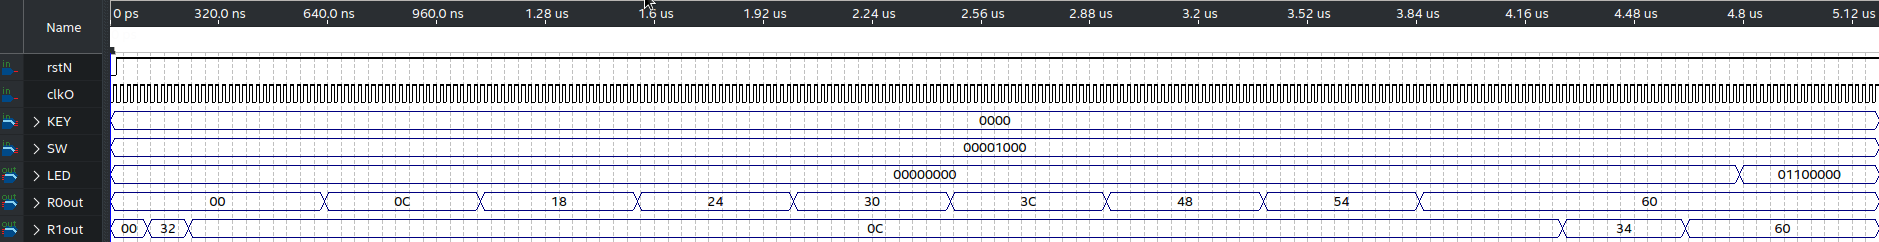
\includegraphics[scale=0.275]{images/8bit_waveform.png}
\caption*{Multiplying by traditional method}
\end{figure}

\begin{figure}[H]
\centering
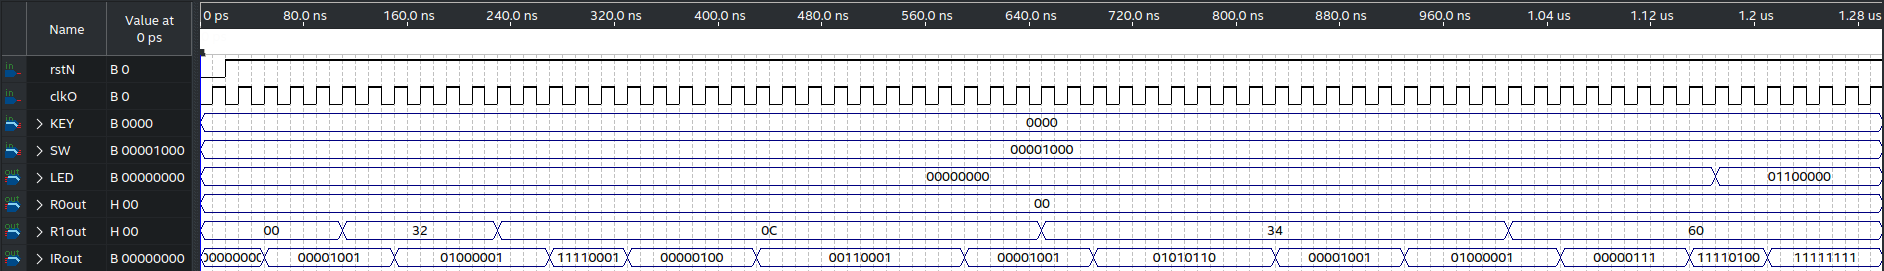
\includegraphics[scale=0.275]{images/8bit_waveform_2.png}
\caption*{Multiplying using logic gates}
\end{figure}

\section{Conclusion}
The processor is way better than the 9-bit processor with larger address width, more specialized instructions. But the tradeoff is the time spent, since most of instructions need two consecutive inputs.

\chapter{Conclusion}
Each processor has its own pros and cons. The 9-bit one can perform faster, but in return, it lack of instructions, small address width. Although the 8-bit processor is slower, it can be widely used thanks to a large set of instructions and the ability to handle large memory.

All of the source code of this subject will be upload on my Github repository, \url{https://github.com/superzeldalink/Digital-Systems-Lab-HCMUT-212}.

\addcontentsline{toc}{chapter}{References}
\begingroup
\let\clearpage\relax
\titlespacing{\chapter}{0pt}{30pt}{10pt}
\begin{thebibliography}{6}
	\bibitem{lab} Department of Electronics, HCMUT, \textit{PreLab, Lab instructions}.
	\bibitem{processor} Wikipedia, \textit{Processor (computing)}, 2022, \url{https://en.wikipedia.org/wiki/Processor_(computing)}
	\bibitem{processor} Wikipedia, \textit{Instruction set architecture}, 2022, \url{
	https://en.wikipedia.org/wiki/Instruction_set_architecture}
	\bibitem{processor} Wikipedia, \textit{MOS Technology 6502}, 2022, \url{https://en.wikipedia.org/wiki/MOS_Technology_6502}
	\bibitem{jdh-8} jdah, \textit{jdh-8}, 2022, \url{https://github.com/jdah/jdh-8}
\end{thebibliography}

\endgroup

\end{document}